\documentclass[11pt,a4paper]{article}
\usepackage[utf8]{inputenc}
\usepackage[T1]{fontenc}
\usepackage[spanish,es-noshorthands]{babel}
\usepackage{lmodern}
\usepackage[margin=2.2cm]{geometry}
\usepackage{amsmath,amssymb}
\usepackage{booktabs,array,graphicx,xcolor,float}
\usepackage[colorlinks=true,linkcolor=blue!50!black,urlcolor=blue!50!black]{hyperref}
\usepackage{enumitem}
\setlist{itemsep=2pt,topsep=4pt}
\newcommand{\lt}{\tilde{\ell}}
\newcommand{\kpar}{\kappa_{\parallel}}
\newcommand{\obs}[1]{\par\smallskip\noindent\colorbox{orange!12}{\parbox{\dimexpr\linewidth-2\fboxsep}{\small #1}}\par\smallskip}

\title{\textbf{Fase 2: sección eficaz y generación de la señal}\\[2pt]\Large Escenario físico: intercambio de $\gamma^*+Z^*$\\[3pt]
\large Reproducción de Sánchez, ACI \textbf{15}(1) 2780 (2023)}
\author{Proyecto \texttt{lw-cms-opendata}}
\date{18 de octubre de 2026}

\begin{document}
\sloppy
\maketitle

\begin{abstract}
\noindent Con el modelo validado en la fase~1 se calculó $\sigma(pp\to\lt^+\lt^-)$ a $\sqrt s=8$~TeV y se generó la señal $\lt\to Ze$, $Z\to jj$ con vértices desplazados (MG5 + Pythia~8, 35\,000 eventos). En esta versión del informe el escenario principal es el \textbf{físicamente correcto}: el $\lt$ tiene carga $-1$, así que se produce por intercambio de $\gamma^*$ \emph{y} $Z^*$. Los resultados principales son:
\begin{enumerate}
\item Con $\gamma+Z$ obtenemos $\sigma=42.3$~fb a 200~GeV, 7.1 veces la del paper, y entre 7 y 9 veces a masas mayores. La Tabla~1 del paper sólo se reproduce omitiendo el fotón (sólo-$Z$, $\pm1\%$). Esa omisión hace que el paper subestime su propia señal; aquí la tratamos como el escenario de \emph{reproducción}.
\item Con $\mathcal{L}=11.5~\mathrm{fb}^{-1}$ se esperan unos 237 eventos de señal a 200~GeV (frente a 33 con la normalización del paper), de los cuales unos 58 tendrían al menos un vértice resoluble tras una selección de tipo paper a nivel de verdad.
\item El $\lt$ de 200~GeV vuela en promedio $\langle L_T\rangle=20~\mu$m, y un 31.5\% de las desintegraciones supera los $20~\mu$m de resolución de vértice de CMS.
\end{enumerate}
Se implementó la geometría acausal reflejando el vértice de desintegración ($\mathrm{SV}'=2\,\mathrm{PV}-\mathrm{SV}$) en los mismos eventos. También quedan resueltas dos ambigüedades del paper: la ventana de 80--160~GeV es sobre $m_{jj}$, y el eje de $\kpar$ está en mm$\cdot$GeV (3D).
\end{abstract}

\section{Organización}
Dos agentes trabajaron en paralelo sin tocar \texttt{model/}:
\begin{itemize}
\item \textbf{A, sección eficaz} (\texttt{generation/xsec/}): unas 90 corridas de MG5 cruzando masas, \texttt{lwRep}, PDFs, escalas, sólo-$\gamma$/sólo-$Z$ y la cadena con $Z\to jj$, más un cálculo analítico LO independiente.
\item \textbf{B, generación} (\texttt{generation/events/}): MG5 con \texttt{time\_of\_flight}, Pythia~8.317 (CUETP8M1) con salida HepMC2, un post-procesador acausal y el análisis a nivel de verdad.
\end{itemize}
Configuración común: \texttt{MeLW}$=5\times10^{-4}$, \texttt{etaLW}$=+1$ (recomendación de la fase~1; se comprobó que $\eta=\pm1$ no cambia $\sigma$, con una diferencia del 0.3\% compatible con la estadística), \texttt{lwRep}$=0$, PDF NNPDF2.3~LO (\texttt{nn23lo1}) y escala dinámica por defecto de MG5.

\section{Sección eficaz}
\begin{table}[H]
\centering\small
\begin{tabular}{c|c|cc|cc}
\toprule
$M_{\lt}$ (GeV) & Paper (fb) & \textbf{Sólo $Z$}, \texttt{lwRep}=0 (fb) & cociente & $\gamma+Z$, \texttt{lwRep}=0 (fb) & $\gamma+Z$, \texttt{lwRep}=1 (fb)\\
\midrule
200 & 5.97 & $\mathbf{5.950}\,^{+4.4\%}_{-4.2\%}$ & 0.997 & $42.30\,^{+3.7\%}_{-3.2\%}$ & 77.05\\
300 & 0.96 & $\mathbf{0.958}\,^{+6.4\%}_{-5.9\%}$ & 0.998 & $7.530\,^{+5.7\%}_{-5.2\%}$ & 13.65\\
400 & 0.23 & $\mathbf{0.2274}\,^{+8.3\%}_{-7.1\%}$ & 0.989 & $1.943\,^{+7.1\%}_{-6.6\%}$ & 3.528\\
500 & 0.06 & $\mathbf{0.0668}\,^{+9.4\%}_{-8.2\%}$ & 1.114 & $0.6136\,^{+8.6\%}_{-7.6\%}$ & 1.115\\
\bottomrule
\end{tabular}
\caption{LO, NNPDF2.3, error estadístico $\sim0.1\%$. Las bandas son de escala ($\mu_{R,F}\times2^{\pm1}$). La dispersión entre PDFs LO de la época (CTEQ6L1, MSTW08LO) añade $+5$--$7\%$ a 200~GeV y $+10$--$18\%$ a 500~GeV.}
\end{table}

\begin{figure}[H]
\centering
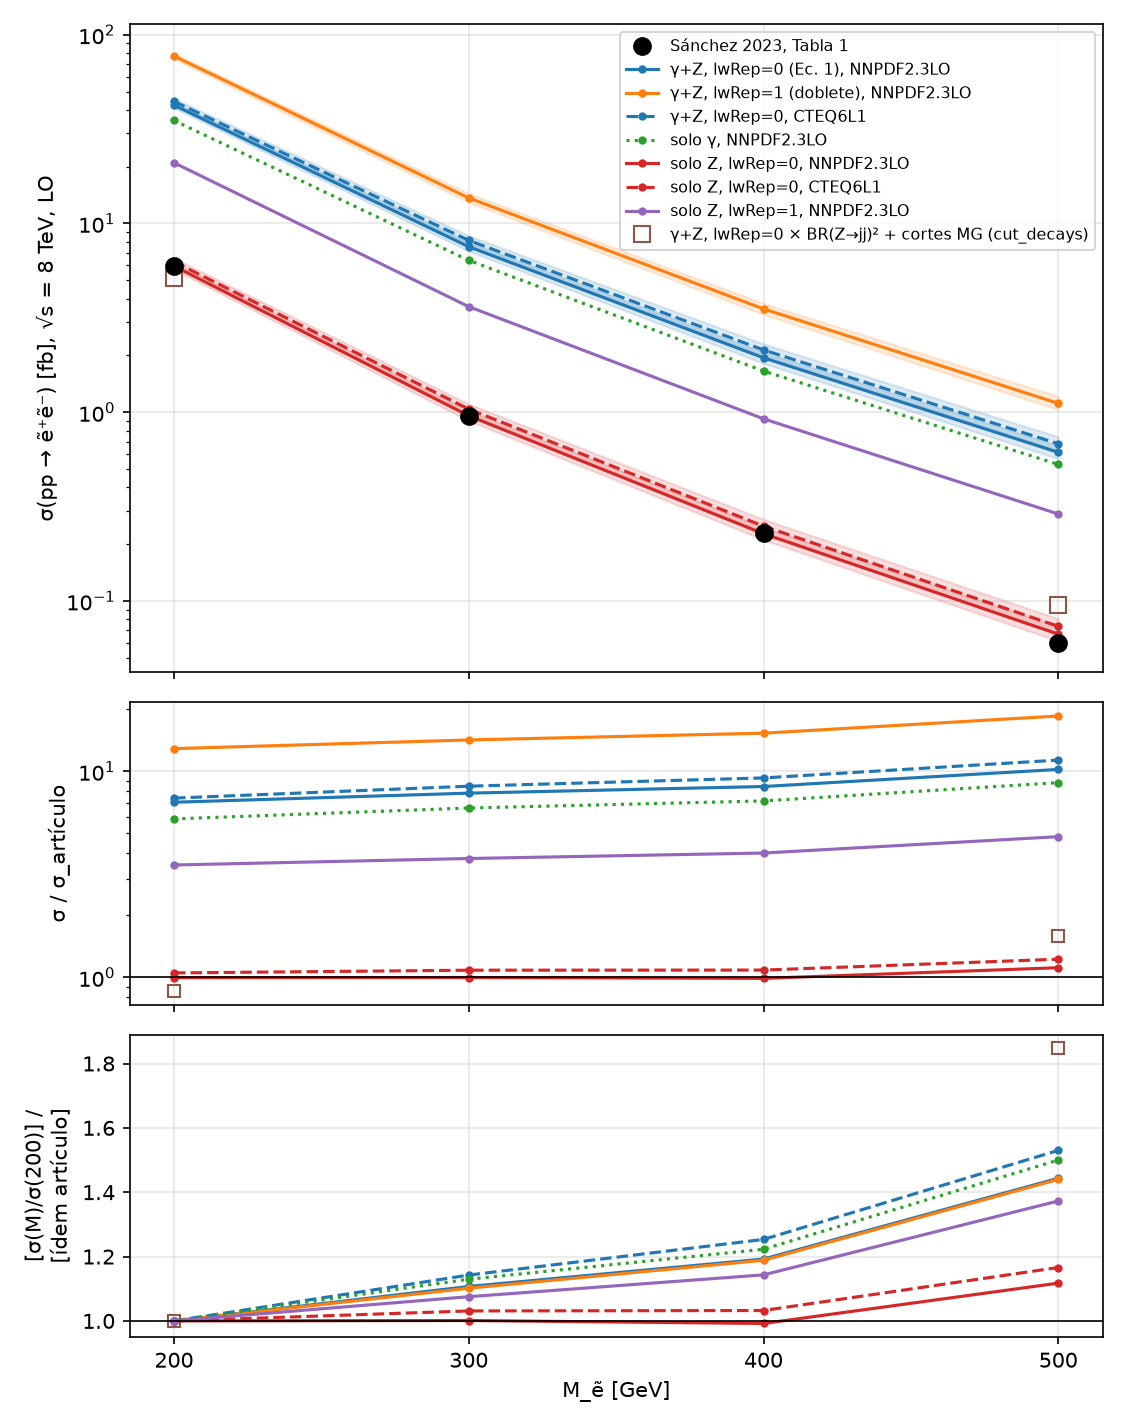
\includegraphics[width=0.62\linewidth]{../generation/xsec/xsec_vs_M.png}
\caption{$\sigma(M)$ para todas las configuraciones, comparadas con la Tabla~1 (puntos negros). Sólo las curvas sólo-$Z$ con \texttt{lwRep}$=0$ (rojas) pasan por los puntos. El panel inferior muestra la forma $\sigma(M)/\sigma(200)$ normalizada a la del paper.}
\end{figure}

\textbf{Qué descarta la dependencia en masa.} El cociente $\sigma(M)/\sigma(200)$ apenas depende del PDF y de la escala:
\begin{itemize}
\item paper: $(1,\,0.161,\,0.0385,\,0.0101)$;
\item sólo-$Z$: $(1,\,0.161,\,0.0382,\,0.0112)$;
\item cualquier configuración $\gamma+Z$: $\approx(1,\,0.178,\,0.046,\,0.0145)$.
\end{itemize}
Por tanto ningún factor constante sobre $\gamma+Z$ (una sola quiralidad, un BR, cortes, otra PDF o escala, 7~TeV) puede reproducir el paper. Todas esas opciones se probaron explícitamente. También se descartó \texttt{lwRep}$=1$, con y sin fotón.

\textbf{Comprobación independiente.} Un cálculo analítico LO con la rejilla de CTEQ6L1 coincide con MG5 al 0.1\%, así que la diferencia está en el modelo del paper y no en el nuestro. Lo más probable es que su modelo FeynRules sólo tuviera los acoplamientos $Z$ de su Ec.~1, que efectivamente no incluye el fotón.

\obs{\textbf{Decisión de normalización (este informe).} El escenario principal es \textbf{$\gamma+Z$}, \texttt{lwRep}$=0$, NNPDF2.3: 42.3, 7.53, 1.94 y 0.614~fb para $M=200$, 300, 400 y 500~GeV. La normalización del paper (sólo-$Z$: 5.95~fb a 200~GeV) se conserva sólo como escenario de reproducción, para comparar con su Fig.~2.
El peso por evento es $w=\sigma\,\mathrm{BR}(Z\to\mathrm{had})^2\,\mathcal{L}/N$, con $\mathrm{BR}=0.6991$ (PDG) y $\mathcal{L}=11.47~\mathrm{fb}^{-1}$.
Una ventaja de este escenario: las muestras generadas ya son $\gamma+Z$, así que su cinemática y su normalización son coherentes sin más supuestos. La comprobación pendiente (si la cinemática sólo-$Z$ coincide con la de $\gamma+Z$) sólo afecta al escenario de reproducción.}

\obs{\textbf{Cadena con $Z\to jj$ en MG5.} Las secciones eficaces de la cadena completa no deben usarse para normalizar:
\begin{itemize}
\item La muestra generada (17.2~fb, sin cortes) es igual a $42.3\times\mathrm{BR}^2\times0.84$. El 0.84 es la pérdida por \texttt{bwcutoff}$=15$, que recorta las cuatro resonancias a $\pm15\Gamma$ ($(2/\pi)\arctan15=0.958$ cada una).
\item Con los cortes por defecto de MG5 (\texttt{cut\_decays}) la cadena da 5.12~fb a 200~GeV, un valor que coincide con el paper por casualidad: la forma en $M$ es incorrecta (1.6 veces el paper a 500~GeV).
\end{itemize}
Por eso normalizamos con $\sigma$ inclusiva $\times\,\mathrm{BR}^2$.}

\section{Generación de la señal}
\begin{itemize}
\item \textbf{MG5:} cadena de desintegración \texttt{(elw$\pm$ > e$\pm$ z, z > qz qz)}, con \texttt{qz} $=u,c,d,s,b$ y sus antiquarks, que conserva las correlaciones de espín LO exactas. Protón de 4 sabores, sin cortes de generador, y \texttt{time\_of\_flight}$=0$, de modo que el LHE lleva el tiempo de vida propio (VTIMUP).
\item \textbf{Pythia~8.317:} \texttt{LesHouches:setLifetime=1}, tune CUETP8M1, MPI/ISR/FSR activados, salida HepMC2 2.06 y jets de verdad anti-$k_T$ 0.5.
\item \textbf{Muestras:} 20k eventos a 200~GeV y 5k en cada una de las otras masas, en versiones causal y acausal, unos 3.2~GB en total (\texttt{generation/events/samples/}).
\end{itemize}

\textbf{Verificación de vértices.}
\begin{itemize}
\item El $\lt$ se desintegra en $\mathrm{SV}=c\tau\,\vec p/m$, que coincide con $\beta\gamma c\tau$ a $10^{-8}$.
\item De 6.4 millones de descendientes estables (todas las masas), \textbf{ninguno} nace en el PV. A 200~GeV, 718k nacen en el SV y 987k más lejos, de desintegraciones secundarias de $\pi^0$, $D$ y $B$.
\item Hay una anomalía menor sin explicar: 66 pasos ``hacia atrás'' de $\le5$~nm dentro del paso partón$\to$cuerda de Pythia, despreciables frente a $20~\mu$m.
\end{itemize}

\textbf{Implementación de la acausalidad.} Siguiendo a Alvarez et al.\ (Ec.~1) y a Grinstein--O'Connell--Wise (0805.2156), el post-procesador \texttt{tools/lw\_reflect\_hepmc.py} desplaza el vértice de cada $\lt$ y todos los vértices descendientes en $\Delta=-2(\mathrm{SV}-\mathrm{PV})$.
\begin{itemize}
\item Los cuadrimomentos quedan idénticos byte a byte, y ningún vértice fuera del árbol del $\lt$ se mueve.
\item El archivo causal y el acausal contienen los mismos eventos (números aleatorios comunes).
\end{itemize}

\section{Resultados a nivel de verdad}
\begin{table}[H]
\centering\small
\begin{tabular}{c|cccc|cc}
\toprule
$M$ (GeV) & $\langle\beta\gamma\rangle$ & $\langle\beta\gamma_T\rangle$ & $\langle L_T\rangle$ ($\mu$m) & $f(L_T>20~\mu\mathrm{m})$ & $f(>20~\mu\mathrm{m})$ tras sel. & $f$(WDVC) tras sel.\\
\midrule
200 & 2.05 & 0.73 & 20.0 & 31.5\% & 33.5\% & 27.4\%\\
300 & 1.58 & 0.67 & 10.7 & 15.5\% & 16.4\% & 13.5\%\\
400 & 1.33 & 0.63 & 7.7 & 8.6\% & 8.2\% & 6.4\%\\
500 & 1.15 & 0.59 & 5.6 & 4.8\% & 4.0\% & 2.9\%\\
\bottomrule
\end{tabular}
\caption{Desplazamiento del $\lt$. ``Tras sel.'' significa después de una selección de tipo paper aplicada a nivel de verdad: electrones con $p_T>40/25$~GeV y $|\eta|<2.5$, jets con $p_T>20$~GeV. La eficiencia de esa selección es del 52\% a 200~GeV.}
\end{table}

\begin{figure}[H]
\centering
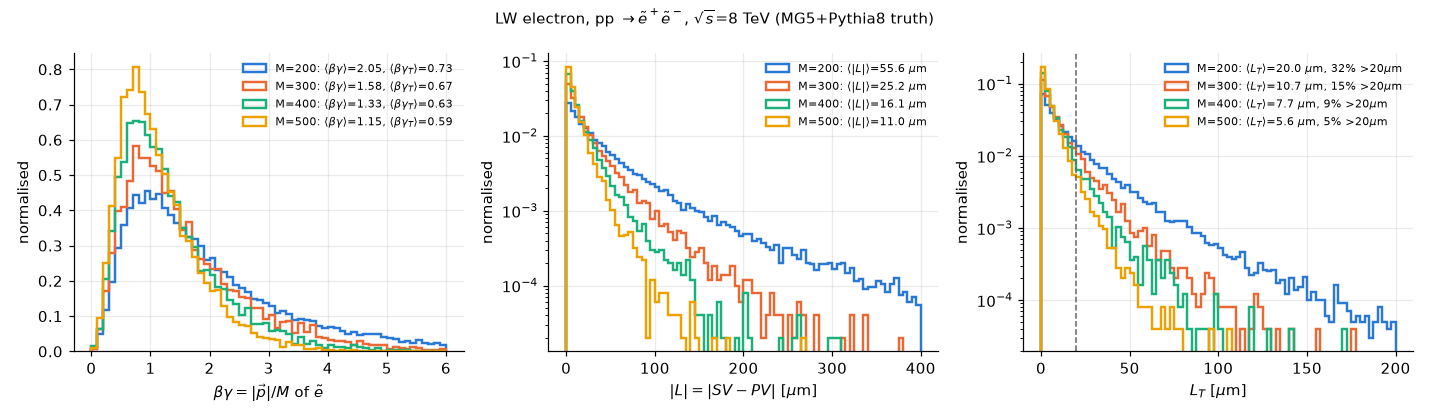
\includegraphics[width=\linewidth]{../generation/events/analysis/plots/displacement_vs_mass.png}
\caption{$\beta\gamma$, $|L|$ y $L_T$ del $\lt$ para cada masa. La línea discontinua marca $20~\mu$m.}
\end{figure}

\begin{itemize}
\item \textbf{Comparación con la fase 1:} a 200~GeV el desplazamiento es mayor que en la estimación burda (31.5\% frente a 15--22\%). El LHE solo ya da $\langle\beta\gamma_T\rangle=0.71$, así que la diferencia viene de la cinemática partónica, no de Pythia.
\item \textbf{Elección de masa:} confirma la elección del paper. A $M\ge400$~GeV menos del 10\% de las desintegraciones es resoluble.
\end{itemize}

\begin{figure}[H]
\centering
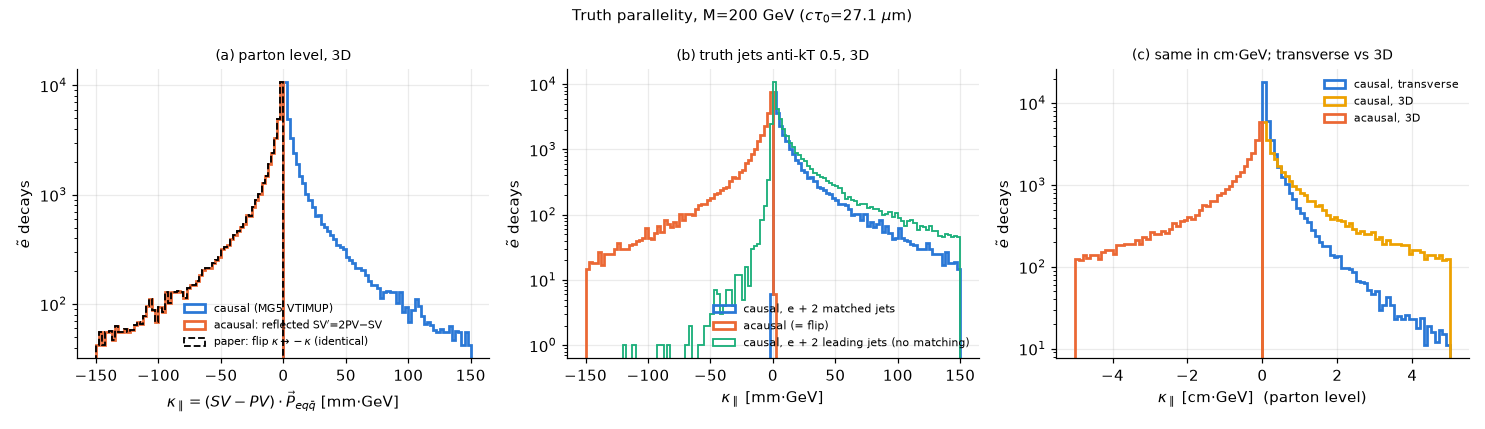
\includegraphics[width=\linewidth]{../generation/events/analysis/plots/kappa_par_M200.png}
\caption{$\kpar$ a nivel de verdad, $M=200$~GeV: (a) a nivel partónico, causal y acausal, con el ``flip'' del paper superpuesto; (b) con jets de verdad; (c) en cm$\cdot$GeV, transversal frente a 3D.}
\end{figure}

\textbf{Paralelidad.}
\begin{itemize}
\item \textbf{Escala:} la mediana causal es 8.5~mm$\cdot$GeV y el percentil 95 es 157~mm$\cdot$GeV. El rango $\pm150$ de la Fig.~2 del paper contiene el 92--95\% de la señal si $\kpar$ está en mm$\cdot$GeV y es 3D. En cm$\cdot$GeV la señal ocuparía unos pocos bins centrales. Concluimos que \textbf{el paper usa mm$\cdot$GeV en 3D}.
\item \textbf{Reflexión frente a flip:} a nivel de verdad la reflexión y el ``flip'' del paper dan el mismo $\kpar$ por construcción. Sólo pueden diferir tras la reconstrucción (ajuste de vértices, cortes respecto al beamspot, asociación traza--PV), que es lo que mediremos en la fase~3.
\item \textbf{Emparejamiento de jets:} con jets emparejados con la verdad, sólo un 0.02\% de las desintegraciones causales tiene $\kpar<0$. Con los dos jets más energéticos sin emparejar, ese porcentaje sube al 8\%: el emparejamiento combinatorio ``diluye'' la asimetría.
\end{itemize}

\begin{figure}[H]
\centering
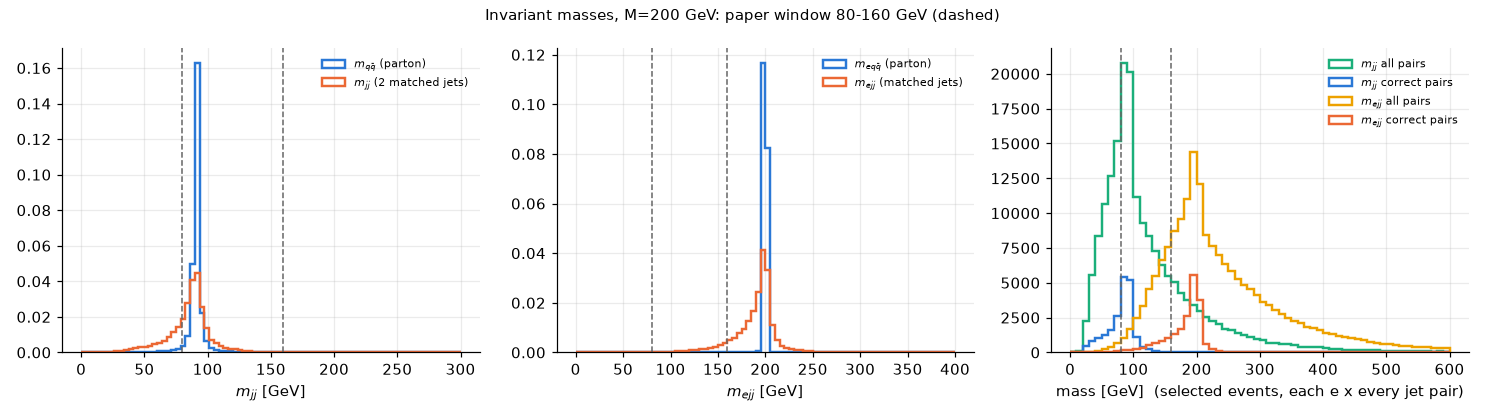
\includegraphics[width=\linewidth]{../generation/events/analysis/plots/masses_M200.png}
\caption{$m_{jj}$ y $m_{ejj}$ a nivel partónico y con jets, frente a la ventana de 80--160~GeV del paper (líneas discontinuas). A la derecha, todas las combinaciones electrón $\times$ par de jets.}
\end{figure}

\textbf{Ventana de masa.}
\begin{itemize}
\item \textbf{Va sobre $m_{jj}$.} La ventana conserva el 72--77\% de los pares de jets correctos. Sobre $m_{ejj}$, que tiene su pico en $\sim195$~GeV, conservaría sólo el 9\% a 200~GeV y menos del 1\% para $M\ge300$~GeV.
\item \textbf{Pureza:} con el emparejamiento del paper (cada electrón con cada par de jets) sólo un 11\% de las combinaciones son correctas. Hay mucho combinatorio.
\end{itemize}

\section{Señal esperada en los datos abiertos de 2012}
\begin{table}[H]
\centering\small
\begin{tabular}{c|cc|c|ccc}
\toprule
 & \multicolumn{2}{c|}{Producidos ($\times\mathrm{BR}^2$)} & & \multicolumn{3}{c}{Escenario $\gamma+Z$}\\
$M$ (GeV) & $\gamma+Z$ & sólo-$Z$ (paper) & $\sigma_{\gamma Z}/\sigma_Z$ & tras sel. & $\lt$ con WDVC & eventos con $\ge1$ WDVC\\
\midrule
200 & 237.1 & 33.4 & 7.1 & 122.9 & 67.3 & 58.1\\
300 & 42.2 & 5.4 & 7.9 & 28.2 & 7.6 & 7.1\\
400 & 10.9 & 1.3 & 8.5 & 7.8 & 1.0 & 1.0\\
500 & 3.4 & 0.4 & 9.2 & 2.5 & 0.1 & 0.1\\
\bottomrule
\end{tabular}
\caption{Número esperado de eventos para $\mathcal{L}=11.47~\mathrm{fb}^{-1}$, con $\mathrm{BR}(Z\to\mathrm{had})^2=0.489$. ``Tras sel.'' es la selección de tipo paper a nivel de verdad. ``WDVC'' es $L_T>20~\mu$m con $p_T$ total $>20$~GeV, por $\lt$. La última columna supone que los dos $\lt$ de un evento son independientes. Todo es a nivel de verdad: faltan la eficiencia de reconstrucción de vértices y los cortes de calidad de la fase~3.}
\end{table}
\begin{itemize}
\item \textbf{Consecuencia para la Fig.~2 del paper:} la señal no tendría que escalarse $\times1000$ sino, como mucho, $\times\sim140$ para verse igual. Aun así la asimetría en $\kpar$ sigue siendo pequeña frente al fondo hasta conocer la eficiencia real de reconstrucción.
\item \textbf{Masa útil:} sólo $M\simeq200$~GeV, y en menor medida 300~GeV, dejan un número de vértices resolubles mayor que 1 con la luminosidad de 2012. Para 400--500~GeV la señal física, incluso con el fotón, es inobservable con estos datos.
\item \textbf{Referencia de literatura:} Alvarez et al.\ obtienen $\sigma$ del mismo orden a 14~TeV con $\gamma+Z$ (66.7~fb a 300~GeV, incluyendo bosones LW a 3~TeV), coherente con que el fotón domine la producción.
\end{itemize}

\section{Parámetros fijados para las fases siguientes}
\begin{center}\small
\begin{tabular}{l>{\raggedright\arraybackslash}p{12cm}}
\toprule
Parámetro & Valor\\
\midrule
Modelo & \texttt{LWElectron\_UFO}: \texttt{MeLW}$=5\times10^{-4}$, \texttt{etaLW}$=+1$, \texttt{lwRep}$=0$\\
PDF / escala & NNPDF2.3~LO (\texttt{nn23lo1}) / dinámica por defecto de MG5\\
Normalización & \textbf{principal: $\gamma+Z$} (42.3~fb a 200~GeV); reproducción: sólo-$Z$ (5.95~fb). Ambas $\times\mathrm{BR}(Z\to\mathrm{had})^2$\\
Benchmark & $M_{\lt}=200$~GeV, $c\tau_0=27.08~\mu$m\\
Señal acausal & reflexión del vértice en HepMC (se conserva además el ``flip'' para comparar)\\
$\kpar$ & 3D, en mm$\cdot$GeV\\
Ventana de masa & $80<m_{jj}<160$~GeV\\
Entrada a CMSSW & HepMC2 descomprimido mediante \texttt{MCFileSource} (el LHE no puede codificar la reflexión)\\
\bottomrule
\end{tabular}
\end{center}

\section{Limitaciones y pendientes}
\begin{enumerate}
\item \textbf{Generador:} Pythia~8 con CUETP8M1, en lugar del Pythia~6 Z2* que usó CMS en 2012. Secciones eficaces LO, sin factor $K$. BR$(\lt\to Ze)=1$, como en el paper (en el LWSM completo sería $\approx0.71$ a 200~GeV).
\item \textbf{Herramientas:} el binding de Python de LHAPDF da segfault, así que no hay errores de PDF por réplicas, sólo la dispersión entre conjuntos. Al conjunto MSTW08LO le faltaban parámetros de $\alpha_s$ en su \texttt{.info}; se añadieron valores de relleno, que no afectan a $\sigma$ LO. El original quedó guardado como \texttt{.orig}.
\item \textbf{Cambio fuera del proyecto:} MG5 actualizó \texttt{input/mg5\_configuration.txt}. La ruta a \texttt{lhapdf\_py3} antes no existía.
\item \textbf{Sin verificar:} la cinemática sólo-$Z$ frente a $\gamma+Z$ (sólo afecta al escenario de reproducción); la diferencia de 11\% a 500~GeV con el paper (posible redondeo); y el comportamiento de CMSSW 5\_3\_32 con HepMC (que el \texttt{VtxSmeared} conserve la reflexión y que Geant4 arranque los productos del $\lt$ en sus SV). Esto último es lo primero que hay que comprobar en la fase~3.
\end{enumerate}

\vspace{4pt}
\noindent\textbf{Cómo repetirlo:} \texttt{generation/xsec/run\_xsec.py} y \texttt{make\_table.py}; \texttt{generation/events/run\_sample.sh}, \texttt{tools/lw\_reflect\_hepmc.py} y \texttt{analysis/truth\_analysis.py}. Los detalles están en los \texttt{README.md} de cada carpeta.
\end{document}
